\documentclass[a4paper]{report}
\usepackage[utf8]{inputenc}
\usepackage{verbatim}
\usepackage{graphicx}

\title{Programming Embedded Systems 2011: Oscilloscope Project}
\author{
	Berglund,Patrik (\texttt{pabe3179@student.uu.se})
\and
	Hansson, Erik (\texttt{erha4253@student.uu.se})
\and
	Hedlund, Markus (\texttt{mahe2599@student.uu.se})
\and
	Söderling, Magnus (\texttt{maso0237@student.uu.se})
}

\begin{document}
\maketitle

\section*{Analysis}
The device is intended to be used by a human operator as a basic oscilloscope
and as a wired network sensor. The input to the device is one or two channels
in the voltage span 0-5V and operator interaction through either touch screen
joystick or network.

\section*{Requirements}
%When used as a stand alone device by an operator the device should have atleast
%3 major modes.
%
The device can be operated as a stand alone by an operator,
or over a network.
%Lite mer om nätverk?
We plan on implementing these modes:
%Är detta förslag om lägen eller ska det vara fyra ovan?
\begin{description}
\item[Normal oscilloscope] \ \\
The measured waveform(s) should be visualised on a display.
The operator shall be able to change certain parameters via a GUI.
The parameters that can be changed are Time/Div(scale of X-axis),
  Voltage/Div(scale of Y axis), choose which of the 2 channels.
  or both to plot.
The possibility to freeze/un-freeze the display should be realised.

\item[Recording] \ \\
In this mode one or both of the channels are recorded for future use.
The sample rate can be adjusted.  

\item[Playback] \ \\
The operator should be able to start playback of recorded data and manipulate
what is output to the display as if it was measured live(in oscilloscope mode).
In Playback mode the user should be able to use the same controllers and features 
as oscilloscope mode with recorded data
%slutet av denna mening är nog inte helt 100%
%Alternativ formulering:
%In Playback mode the user should be able to use the same controllers and features 
%as in oscilloscope mode but with recorded data.  

\item[Voltage-meter mode] \ \\
The current AC/DC voltage measured from one or two channels should be
displayed as digits.

\end{description}
When used as a network-sensor data should be transmitted to a client.

\section*{Architecture}
A development board with a touch capable LCD display, buttons and network port
will be used to realise the product.
Probes for measuring voltages will be needed.
The software will be implemented using the FreeRTOS operating system.
\pagebreak
\subsection*{Software modules}
A rough sketch of which software modules need to be implemented. 
Since we are using a multi-tasking operating system every module
will most likely be implemented as separate tasks.
\begin{figure}[h!]
	\centering
	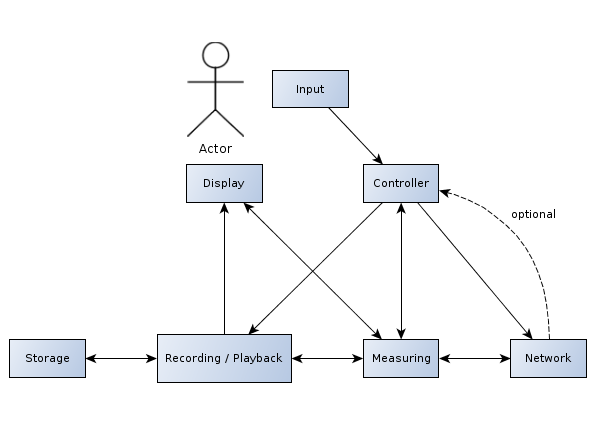
\includegraphics[width=0.9\textwidth]{software_modules.png}
	\caption{Software modules and dependencies.}
\end{figure}
\begin{description}
\item [Measuring] Collects measurements from sensors.
\item [Display] Basic graphics, menus and plotting.
\item [Input] Interaction with the user via buttons and touch screen.
\item [Network] Transmits the current sensor value to interested clients.
\item [Recording/playback] Extreme high/low speed measurement.
\item [Storage] Backend for recording module.
\end{description}

\section*{Messages}
\begin{tabular}{ l | l | l }
  \textbf{Name} & \textbf{Arguments} & \textbf{Comments} \\ \hline
  \texttt{SUBSCRIBE} & Channel, Destination & FOO \\
  \texttt{UNSUBSCRIBE} & Channel, Destination & FOO \\
  \texttt{DATA} & Value, Id, Channel & FOO \\
  \texttt{SET\_SAMPLE\_RATE} & Channel, Rate & FOO \\
  \texttt{GET\_SAMPLE\_RATE} & Channel, Dest & FOO \\
\end{tabular}

% Nedan är sådant vi vill klä i ord ovan (de vi inte har gjort)?
\begin{comment}
\section*{Idea sketch}
BASIC
2 channel oscilloscope with possibility to freeze frame using a screen tap.
adjustments for time/voltage-div.
// adjustment of samplerate.
Recording and playback maybe using higer sample rate for recording?

DC voltage displayed using numbers(min/max reset).
AC voltage displayed using numbers(min/max reset).

NETWORK
Sensor sending raw data through apropriate protocol.



EXTRA
Trace (last sweep fading).
Trigger sweep(level).
Filters (FFT).
Use sensor as filter, output a filtered signal.

http-server displaying images or data.
...
\end{comment}
\end{document}
